\documentclass[10pt]{beamer}

\usetheme{metropolis}
\usepackage{appendixnumberbeamer}

\usepackage{booktabs}
\usepackage[scale=2]{ccicons}
\usepackage{graphicx}
\usepackage{hyperref}
\usepackage{circuitikz}
\usepackage{pdflscape}
\usepackage{smartdiagram}

\usepackage{color}
\usepackage{listings}

\lstset{
	basicstyle=\footnotesize\ttfamily,
    keepspaces=true,
    showstringspaces=false,
    language=PHP,
    commentstyle=\ttfamily,
}

\usepackage[OT4]{polski}
\usepackage[utf8]{inputenc}

\usepackage{pgfplots}
\usepgfplotslibrary{dateplot}

\usepackage{xspace}
\newcommand{\themename}{\textbf{\textsc{metropolis}}\xspace}

\setbeamertemplate{frame footer}{}
\setbeamertemplate{frame numbering}{}

\usetikzlibrary{shapes,arrows}

\tikzstyle{decision} = [diamond, draw, fill=blue!20, 
    text width=4.5em, text badly centered, node distance=3cm, inner sep=0pt]
\tikzstyle{block} = [rectangle, draw, fill=blue!20, 
    text width=5em, text centered, rounded corners, minimum height=4em]
\tikzstyle{line} = [draw, -latex']
\tikzstyle{cloud} = [draw, ellipse,fill=red!20, node distance=3cm,
    minimum height=2em]


\title{Inne wzorce architektoniczne}

\subtitle{Projektowanie i programowanie systemów internetowych I}
\author{mgr inż. Krzysztof Rewak}
\date{\today}
\institute{Wydział Nauk Technicznych i Ekonomicznych \\ Państwowa Wyższa Szkoła Zawodowa im. Witelona w Legnicy}

\begin{document}

\maketitle

\begin{frame}{Plan prezentacji}
  \setbeamertemplate{section in toc}[sections numbered]
  \tableofcontents[hideallsubsections]
\end{frame}


\section{MVC}

\begin{frame}{Czy MVC to remedium na wszystko?}
	Nie.
\end{frame}

\section*{Podsumowanie}

\begin{frame}{Czy MVC to remedium na wszystko?}
	MVC, nie dość, że bardzo często źle rozumiane, jest również bardzo często źle wykorzystywane.
	
	Często też uważa się, że jest odpowiedzią na każdy architektoniczny problem.
\end{frame}

\begin{frame}[fragile]{MVC}
	\hspace*{1.25cm}%
	\begin{tikzpicture}[node distance=4cm, minimum size=2cm, auto]
	
		\node [circle, fill=orange,inner sep=3pt] (user) {użytkownik};
		
		\node [block, above right of=user] (controller) {kontroler};
		\node [block, above left of=user] (view) {widok};
		\node [block, above left of=controller] (model) {model};
		
	
		\path [line] (user) -- node[label={[shift={(2,-3.5)}]wywołuje}] {} (controller);
		\path [line] (controller) -- node[label={[shift={(2,-0.5)}]żąda zmian}] {} (model);
		\path [line] (model) -- node[label={[shift={(-2,-0.5)}]uaktualnia}]  {} (view);
		\path [line] (view) -- node[label={[shift={(-2,-3.5)}]wyświetla}] {} (user);
	\end{tikzpicture}
\end{frame}

\begin{frame}{MVC}
	\textbf{Model} odpowiada za... mapowanie danych? Niekoniecznie. Niektórzy autorzy wręcz mówią, że modelem jest cała warstwa domeny projektu.
\end{frame}

\begin{frame}{MVC}
	\textbf{Widok} to praktycznie rzecz biorąc wystawienie danych. Zazwyczaj myślimy o zbudowanym HTML-u, ale czy odpowiedź JSON też będzie widokiem?
\end{frame}

\begin{frame}{MVC}
	\textbf{Kontroler} natomiast powinien tylko i wyłącznie odebrać żądanie, przekazać je modelowi (w jakikolwiek sposób podzielonemu na warstwy!) i zwrócić znów użytkownikowi.
\end{frame}

\begin{frame}{MVC}
	Większość współczesnych frameworków webowych stosuje (albo nazywa inkorporuje do nazwy) wzorzec MVC. Czasami jednak trzeba sięgnąć po coś więcej, aby zbudować coś lepiej.
\end{frame}

\section{IoC}

\begin{frame}{Odwrócenie sterowania}
	\textbf{\emph{Inversion of Control}}, czyli \emph{odwrócenie sterowania} polega na "przeniesieniu funkcji sterowania wykonywaniem programu do używanego frameworku".
\end{frame}

\begin{frame}{Dekonstrukcja definicji}
	\emph{Klasyczne} podejście do programowania obiektowego polega na tworzeniu nowych obiektów i wywoływaniu na nich metod.
	
	Programista kodując steruje zachowaniem programu.
\end{frame}

\begin{frame}{Dekonstrukcja definicji}
	IoC polega na tym, że dostarczony framework steruje programem, a programista jedynie podłącza się w odpowiednim momencie.
\end{frame}

\begin{frame}{Zasada Hollywood}
	\emph{Nie dzwoń do nas. My oddzwonimy do ciebie.}
\end{frame}

\begin{frame}{Wstrzykiwanie zależności}
	Najpopularniejszą implementacją odwrócenia sterowania jest wstrzykiwanie zależności. 
	
	Należy pamiętać, że pojęcia te nie są tożsame.
\end{frame}

\begin{frame}[fragile]{Wstrzykiwanie zależności}
	Przy okazji omawiania testowania przedstawiono przykład różnych implementacji testowania; która jest nalepsza?

\begin{lstlisting}
public function send(): void {
    $mailer = new Mailer;
    $mailer->send();
}
\end{lstlisting}

	czy może:

\begin{lstlisting}
public function send(Mailer $mailer): void {
    $mailer->send();
}
\end{lstlisting}

	czy może:

\begin{lstlisting}
public function send(MailerInterface $mailer): void {
    $mailer->send();
}
\end{lstlisting}
\end{frame}

\begin{frame}{Wstrzykiwanie zależności}
	Dzięki IoC możemy uniezależnić wykonanie zadania od jego implementacji. Na poziomie wyższej warstwy zostanie stworzony obiekt implementujący odpowiedni interfejs i przekazany do kontrolera, serwisu lub innej wykonawczej klasy.
\end{frame}

\begin{frame}{Plusy?}
\begin{itemize}
	\item SOLID-nie porządkuje kod;
	\item zwiększa elastyczność naszego oprogramowania;
	\item zmniejsza możliwość wywołania efektów ubocznych czy modyfikacjach;
	\item ułatwia testowanie.
\end{itemize}
\end{frame}

\begin{frame}{Minusy?}
\begin{itemize}
	\item zwiększa skomplikowanie kodu?
\end{itemize}
\end{frame}

\begin{frame}{Życie po wstrzykiwaniu zależności}
	Co jeszcze jest implementacją IoC?

\begin{itemize}
	\item wzorzec lokalizatora usług (\emph{service locator})
	\item operacyjny wzorzec metody szablonowej (\emph{template method})
	\item operacyjny wzorzec strategii (\emph{strategy})
\end{itemize}

	O wszystkich będzie mowa na przyszłosemestralnych zajęciach \emph{Zaawansowane metody programowania}.
\end{frame}

\section{ETL}

\begin{frame}{ETL}
	\textbf{ETL}, \emph{extract, transform, load} (ang. \emph{pobierz, zmień, wgraj}) to kolejny przydatny w biznesie wzorzec architektoniczny.
\end{frame}

\begin{frame}{ETL}
	\begin{figure}[t]
		\centering
		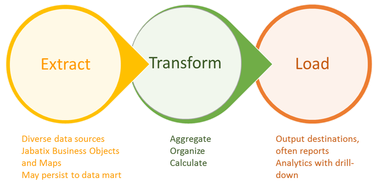
\includegraphics[width=.75\linewidth]{etl.png}
		\caption{\url{https://jabatixde.wordpress.com/2017/03/10/private-basic-pattern-high-value-extract-transform-load-with-jabatix/}}
	\end{figure}
\end{frame}

\begin{frame}{\emph{Extract}}
	\textbf{Extract} polega na przyjęciu w dowolny sposób danych wejściowych.
\end{frame}

\begin{frame}{\emph{Transform}}
	\textbf{Transform} polega na ustandaryzowaniu danych wejściowych wedle wybranego schematu.
\end{frame}

\begin{frame}{\emph{Load}}
	\textbf{Load} polega na przesłaniu ustandaryzowanych danych dalej.
\end{frame}

\begin{frame}{ETL}
	\textbf{ETL} zatem może służyć jako system łączący inne systemy i dokładnie w tym celu jest często implementowany.
\end{frame}

\begin{frame}{ETL + IoC?}
	Ciekawym rozwiązaniem może być zastosowanie wzorca strategii przy ETL, żeby stworzyć system bramek API.
\end{frame}

\begin{frame}{ETL}
	\begin{figure}[t]
		\centering
		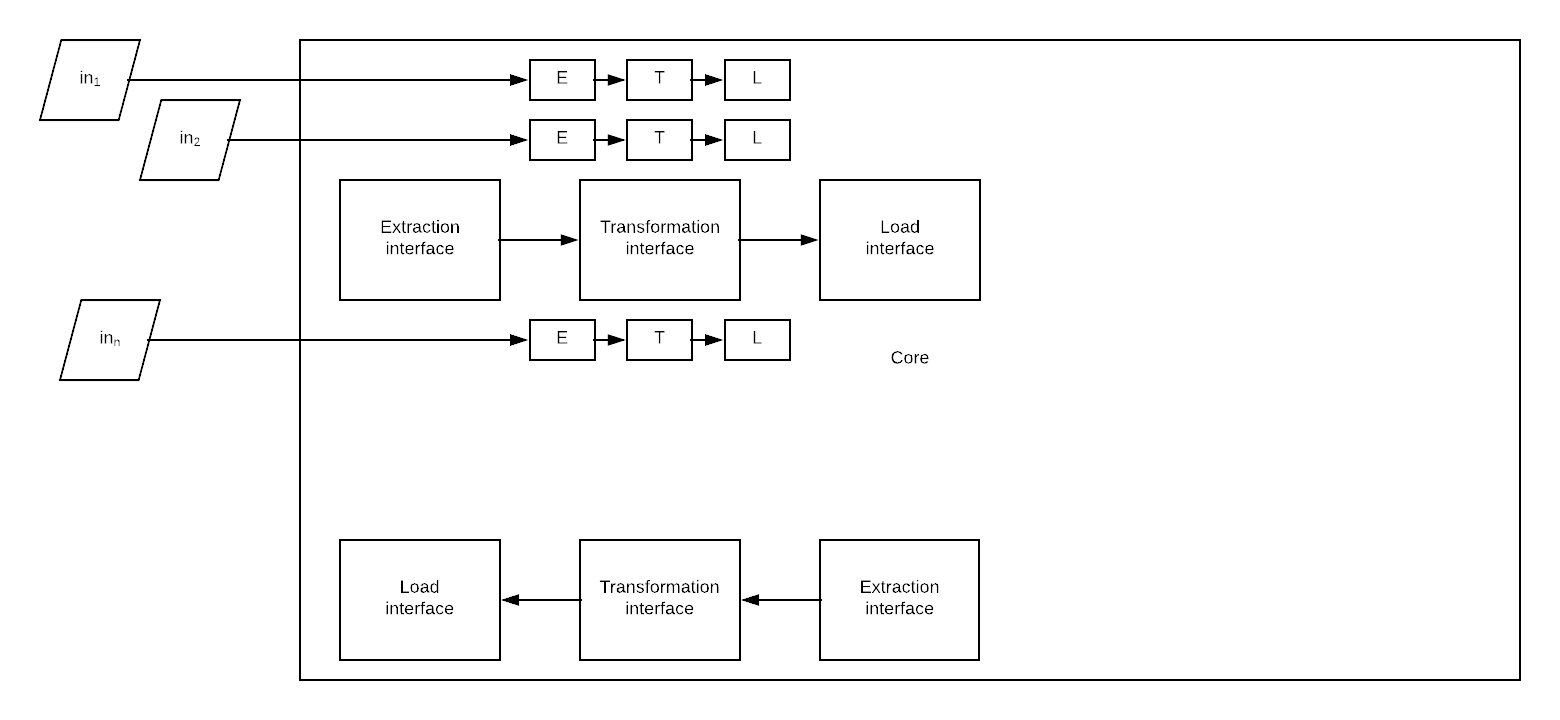
\includegraphics[width=\linewidth]{etls.png}
	\end{figure}
\end{frame}

\section{CQS/CQRS}

\begin{frame}{CQS}
	\textbf{CQS}, \emph{Command Query Separation} (ang. \emph{odseparowanie zapytań od poleceń}) to bardziej metoda programowania niż osobno zdefiniowany wzorzec architektoniczny, ale ostatnimi czasy stała się bardzo modna, więc warto pokrótce o niej wspomnieć.
\end{frame}

\begin{frame}{CQS}
	\textbf{Command} to metoda zmieniająca stan aplikacji, natomiast \textbf{Query} to metoda zwracająca stan aplikacji.
\end{frame}

\begin{frame}{CQS}
	\emph{Pytanie nie powinno zmieniać odpowiedzi.}
\end{frame}

\begin{frame}[fragile]{(nie)CQS}
\begin{lstlisting}
public Response create(string id) {
    User user = Users.create(id);
    return response(user);
}
\end{lstlisting}
\end{frame}

\begin{frame}[fragile]{CQS}
\begin{lstlisting}
public void create(string id) {
    Users::create(id);
}

public Response get(string id) {
    return response(Users.find(id));
}
\end{lstlisting}
\end{frame}

\begin{frame}{CQRS}
	\textbf{CRS}, \emph{Command Query Responsibility Segregation} (ang. \emph{segregacja odpowiedzialności zapytań i poleceń}) to rozszerzenie CQS polegające na tworzeniu nie tylko metod, ale całych klas odpowiedzialnych za zapytania i polecenia.
\end{frame}

\begin{frame}{CQRS}
	\begin{figure}[t]
		\centering
		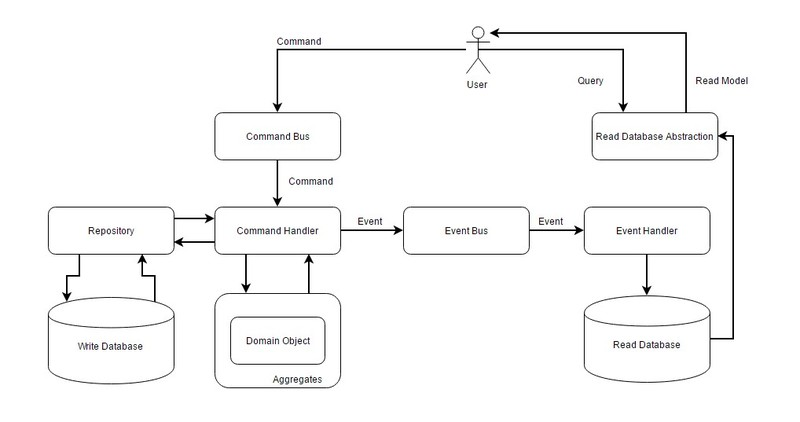
\includegraphics[width=\linewidth]{cqrs.jpg}
	\end{figure}
\end{frame}

\section{Podsumowanie}

\begin{frame}{Bibliografia i ciekawe źródła}
  
	\begin{thebibliography}{9}
		
		\bibitem{gof}
		Gamma, Helm, Johnson, Vlissides, \emph{Design Patterns: Elements of Reusable Object-Oriented Software}, 1994
		
		\bibitem{commitandrun}
		\url{http://commitandrun.pl/2016/05/30/Brutalne_prawdy_o_MVC/}
		
		\bibitem{ioc}
		\url{https://pl.wikipedia.org/wiki/Odwrócenie\_sterowania}
		
		\bibitem{ioc2}
		\url{https://www.sitepoint.com/inversion-of-control-the-hollywood-principle/}
		
		\bibitem{cqrs}
		\url{https://bulldogjob.pl/articles/122-cqrs-i-event-sourcing-czyli-latwa-droga-do-skalowalnosci-naszych-systemow}
	
	\end{thebibliography}

\end{frame}

\appendix

\begin{frame}[standout]
	Pytania?
\end{frame}

\begin{frame}{}

	Kod prezentacji dostępny jest w repozytorium git pod adresem \texttt{https://bitbucket.org/krewak/pwsz-ppsi} \\ \ \\

	\begin{figure}
		\centering
		\href{https://bitbucket.org/krewak/pwsz-ppsi}{
			
\includegraphics[width=.15\textwidth]{../_template/bitbucket.png}
		}
	\end{figure}
	
	Wszystkie informacje dot. kursu dostępne są pod adresem \texttt{http://pwsz.rewak.pl/kursy/4} \\ \ \\

	\begin{figure}
		\centering
		\href{http://pwsz.rewak.pl/kursy/3}{
			
\includegraphics[width=.15\textwidth]{../_template/rewak.png}
		}
	\end{figure}

\end{frame}

\end{document}
